\PassOptionsToPackage{usenames,dvipsnames,table,x11names}{xcolor}
\documentclass[10pt]{article}

%------------------------------------------------------
%                Math Packages
%------------------------------------------------------

%\usepackage[intlimits]{amsmath}
\usepackage{amsmath}
\usepackage{amssymb}
\usepackage{amsthm}
%\everymath{\displaystyle}
\usepackage{siunitx} % for SI units (e.g. C, degree)
\usepackage{bm} % bold for some math symbols
\usepackage{nicefrac} % for nicer fractions sometimes
\usepackage[thinc]{esdiff} % for derivatives
\usepackage{mathtools}

%------------------------------------------------------
%                Tikz and Pgfplots
%------------------------------------------------------

\usepackage{pgfplots}
\usepackage{tkz-euclide}
\pgfplotsset{compat=1.15}
\usetikzlibrary{arrows,shadows,positioning, calc, decorations.markings, hobby, quotes, angles, decorations.pathreplacing, intersections, matrix,backgrounds}
\usepgfplotslibrary{polar,colormaps,fillbetween}
\usepgflibrary{shapes.geometric}
%\usetkzobj{all}

%------------------------------------------------------
%                Formatting
%------------------------------------------------------

% COLORS ----------------------------------------------
%\usepackage[dvipsnames, table]{xcolor}
\usepackage{xcolor}

% FIGURES ---------------------------------------------
\usepackage{graphicx} % for importing images
\usepackage{subcaption} % for making subfigures
\usepackage[labelfont=bf]{caption} % changing style of figures

% PAGE LAYOUT -----------------------------------------
%\linespread{1.3} % changes line spacing

\usepackage[a4paper, portrait, margin=1in]{geometry} % for changing layout of document
%\usepackage[a4paper, portrait, left=0.75in, right = 0.75in, top = 1in, bottom=1in]{geometry}

%\usepackage{indentfirst}
%\usepackage{parskip} % for not indenting paragraphs first
\usepackage{multirow} % having multiple rows
\usepackage{multicol} % having multiple columns
\renewcommand\labelitemi{$\vcenter{\hbox{\tiny$\bullet$}}$} % making bullets in \enumerate smaller
\usepackage[T1]{fontenc} % can combine \sc and \bf font

% LINKS -----------------------------------------------
\usepackage{etoolbox}
\makeatletter % <================================================
\patchcmd{\maketitle}%
  {\def\@makefnmark{\rlap{\@textsuperscript{\normalfont\@thefnmark}}}}%
  {\def\@makefnmark{\rlap{\@textsuperscript{\normalfont\color{blue}\@thefnmark}}}}%
  {}%success
  {}%failure
\makeatother % <=================================================
% for changing color of \thanks{} in title

\usepackage[hidelinks]{hyperref}
\hypersetup{
    colorlinks=true,
    linkcolor=black,
    filecolor=magenta,      
    urlcolor=SteelBlue3,
    citecolor=black,
}

% LANGUAGES -------------------------------------------
\usepackage[english]{babel} % for correctly using english
\usepackage[utf8x]{inputenc} % compiling correctly
\usepackage{CJK} % using Chinese, Japanese, and Korean

% MISC ------------------------------------------------
\usepackage[normalem]{ulem} % for \sout
\usepackage{tikzsymbols} % for emojis
\usepackage{booktabs,eqparbox} % for tables
\usepackage{verbatim} % for verbatim environment

%------------------------------------------------------
%                Custom Commands
%------------------------------------------------------

\newcommand{\done}{\hfill $\square$}
\newcommand{\csch}{\mathrm{csch}}
\newcommand{\sech}{\mathrm{sech}}

%\newcommand{\dd}{\mathop{}\,\mathrm{d}}
\newcommand{\dd}{\,\mathrm{d}}

% COLOR CODING -----------------------------------------------
\newcommand{\code}[1]{\textcolor{Bittersweet}{\texttt{#1}}} % using for emphasizing variables, code, etc.
\newcommand{\mydef}[1]{\textcolor{SteelBlue3}{\textit{#1}}} % defining something

% VENN DIAGRAMS ----------------------------------------------
\def\firstcircle{(90:1.75cm) circle (2.5cm)}
\def\secondcircle{(210:1.75cm) circle (2.5cm)}
\def\thirdcircle{(330:1.75cm) circle (2.5cm)}
\def\sampspace{(-6,-4.25) rectangle (6,5)}  %Cartesian
%\def\sampspace{(225:7cm) rectangle (45:7cm)} %polar

% TO DO LIST -------------------------------------------------
\usepackage{enumitem}

\newlist{todolist}{itemize}{2}
\setlist[todolist]{label=$\square$}

\usepackage{pifont}
\newcommand{\cmark}{\ding{51}}%
\newcommand{\xmark}{\ding{55}}%
\newcommand{\fin}{\rlap{$\square$}{\raisebox{2pt}{\color{Green}{\large\hspace{1pt}\cmark}}}%
\hspace{-2.5pt}}
\newcommand{\wontfix}{\rlap{$\square$}{\color{red}{\large\hspace{1pt}\xmark}}}

% LADE STUFF -------------------------------------------------
\xdef\defsize{4}
\xdef\cursize{5}
\newcommand{\myscale}[1]{\defsize/#1}

%------------------------------------------------------
%                Custom Environments
%------------------------------------------------------

\usepackage{mdframed}

% EXERCISE -------------------------------------------------
\mdfdefinestyle{exercise}{
	backgroundcolor=black!10,roundcorner=8pt,hidealllines=true,nobreak
}

%\begin{mdframed}[style=exercise]
%\end{mdframed}

% MATHEMATICA ------------------------------------------------
\mdfdefinestyle{mathematica}{
	backgroundcolor=Tan!15,roundcorner=8pt,hidealllines=true,nobreak,fontcolor=Bittersweet
}

% R ---------------------------------------------------------
\mdfdefinestyle{R}{
	backgroundcolor=SteelBlue3!10, roundcorner=8pt, hidealllines=true, nobreak, fontcolor=SteelBlue4
}

% R ---------------------------------------------------------
\mdfdefinestyle{python}{
	backgroundcolor=Green!15, roundcorner=8pt, hidealllines=true, nobreak, fontcolor=Green
}

%------------------------------------------------------
%                      Layout
%------------------------------------------------------

% FORMATTING TITLES -----------------------------------
\usepackage{titlesec}
\titleformat*{\section}{\Large \bfseries} % changing section format
\titleformat*{\subsection}{%\color{SteelBlue3} 
\large \bf} % changing subsection format
%\setcounter{secnumdepth}{0} % sets title counter to 0

% PAGE HEADINGS ----------------------------------------------
\usepackage{fancyhdr}

\pagestyle{plain}
\fancyhf{}
\lhead{}
\chead{}
\rhead{}
\cfoot{{ \thepage}}

\renewcommand{\headrulewidth}{0.2pt}
\renewcommand{\footrulewidth}{0pt}
%\pagenumbering{gobble}

%%%%%%%%%%%%%%%%%%%%%%%%%%%%%%%%%%%%%%%%%%%%%%%%%%%%%%%
%%%%%%%%%%%%%%%%%%%%%%%%%%%%%%%%%%%%%%%%%%%%%%%%%%%%%%%
\begin{document}

%------------------------------------------------------
%                       Title
%------------------------------------------------------

\title{\Large \textbf{Singular Value Decomposition}}
\author{{\large  Aiden Kenny}\\
{\large \it Franklin \&{} Marshall College}\\
{\large \it Summer 2019}}
\date{}
\maketitle

%------------------------------------------------------
%                      Document
%------------------------------------------------------

\section{Introduction}

The purpose of this paper is to provide a comprehensive overview of the \mydef{singular value decomposition} (SVD) of a matrix. Any $n \times p$ matrix $\mathbf{A}$ can be decomposed into three separate matrices, given as 
\begin{align}
    \mathbf{A} = \mathbf{U} \mathbf{S} \mathbf{V}^T, \label{eq1}
\end{align}
where $\mathbf{U}$ is an $n \times n$ orthogonal matrix, $\mathbf{S}$ is an $n \times p$ diagonal matrix, and $\mathbf{V}$ is a $n \times n$ orthogonal matrix. 

We could continue to discuss the properties of the three matrices in (\ref{eq1}), but I believe it is important to ensure that the reader has a solid foundation in the necessary theory and terminology needed. For this reason, section 2 provides various linear algebra pre-requisites needed to understand the SVD. It is not until section 3 that (\ref{eq1}) is explored further from a theoretical perspective. Section 4 describes a systematic approach to determining the SVD of a matrix, as well as various computational methods. 

\section{Linear Algebra: Notation and Methods}

In this section we have a brief review of the theory of several linear algebra topics relative to SVD. Note that this review is in no way comprehensive or flushed-out, as that would lead us too far astray from the goal of this paper. For example, topics such as elementary operations or inverse matrices, which are extremely important for linear algebra as a whole, or the idea of treating a matrix as a linear transformation, are completely ignored. 

\subsection{Vectors and Matrices}

For a positive integer $n$, a \mydef{vector} (or \mydef{$n$-vector}) is an ordered list (known as an \mydef{array}) of $n$ numbers, called \mydef{elements} or \mydef{scalars}. The \mydef{order} of a vector is the number of elements it contains, so an $n$-vector has an order of $n$. We will generally denote a vector using a lowercase boldface letter
%\footnote{Some authors, such as Gentle in \cite{MR3645468}, simply denote a vector as a lowercase letter, omitting the boldface. Alternatively, some authors, such as Hastie in \cite{MR2722294}, generally omit the boldface as well, but sometimes use boldface to denote a vector with $n$ elements. This is to help them, for example, distinguish between the row vectors $x_i$ and the column vectors $\mathbf{x}_i$ of the data matrix $\mathbf{X}$. For this paper, I chose to always use boldface so we do not confuse vectors with scalars.}
, e.g. $\mathbf{v}$. The $i^{\text{th}}$ element in $\mathbf{v}$ is denoted using a lowercase letter (the same letter that denotes the vector), e.g. $v_i$ is the $i^{\text{th}}$ element of $\mathbf{v}$). For our purposes, we will assume that the elements of a vector are all real numbers; that is, $v_i \in \mathbb{R}$ for all $v_i$. The notation $\mathbb{R}^n$ is used to denote all $n$-vectors with real elements. 

When we want to express the specific elements of a vector, it is written as either  
\begin{align}
    \mathbf{v} = \begin{pmatrix}
        v_1 \\ \vdots \\ v_n
    \end{pmatrix} \label{eq2}
\end{align}
or 
\begin{align}
    \mathbf{v} = (v_1, \ldots, v_n). \label{eq3}
\end{align}
Vectors are, by default, thought of as ``columns,'' so (\ref{eq2}) seems more natural in that sense. However, for notational purposes, it is often easier to express vectors in the form of (\ref{eq3}). %We will return to this topic momentarily. 
Geometrically, an $n$-vector may be thought of as a point in $n$-dimensional space, where each element of the matrix is the coordinate along one of the axis. 

%Vectors, as well as many others topics covered in Section 2, have very nice geometric interpretations that I believe are extremely helpful for understanding. A vector can be though of as a point in $n$-dimensional space. For example, consider the $2$-vector $\mathbf{v} = (1,2)$. This vector is a point in 2-dimensional space, where the first element is the coordinate along the $x$-axis and the second element is the coordinate along the $y$-axis.

An \mydef{$n \times p$ matrix} is a 2-dimensional array of numbers, with $n$ \mydef{rows} and $p$ \mydef{columns}. The numbers $n$ and $p$ denote the \mydef{shape} of the matrix; if a matrix has the same number of rows and columns (i.e. $n = p$), then the matrix is said to be \mydef{square}. We will denote a matrix using a capital boldface letter, e.g. $\mathbf{A}$. We sometimes also wish to denote a matrix as $\mathbf{A}_{n \times p}$, to indicate the shape of the matrix at a glace. To denote an element in the $i^{\text{th}}$ row and $j^{\text{th}}$ column of a matrix, we use a lowercase letter (the same letter that denotes the matrix) combined with two subscripts $i$ and $j$, e.g. $a_{i,j}$ is the element in the $i^{\text{th}}$ row and $j^{\text{th}}$ column of the matrix $\mathbf{A}$. We again assume that the elements of a matrix are all real numbers. The notation $\mathbb{R}^{n \times p}$ is used to denote all $n \times p$ matrices with real elements. 

When we want to express the specific elements of a matrix, it is written as either 
\begin{align}
    \mathbf{A} = \begin{pmatrix}
        a_{1,1} & \cdots & a_{1,n} \\
        \vdots & \ddots & \vdots \\
        a_{p,1} & \cdots & a_{n,p}
    \end{pmatrix} \label{eq4}
\end{align}
or 
\begin{align}
    \mathbf{A} = (a_{i,j}), \label{eq5}
\end{align}
for $i \in \{ 1,\ldots,n \}$ and $j \in \{ 1,\ldots,p \}$. 

Two matrices are equal only if they have the same shape and the corresponding elements of each matrix are equal. So, for two matrices $\mathbf{A}_{n \times p}$ and $\mathbf{B}_{m \times q}$ to be equal, it must be true that $n = m$, $p = q$, and $a_{i,j} = b_{i,j}$ for all $i \in \{ 1,\ldots,n \}$ and $j \in \{ 1,\ldots,p \}$.

\subsubsection{Relationship Between Vectors and Matrices}
%maybe add info about geometric intuition, linear transformations.
There is a close relationship between vectors and matrices. A \mydef{column vector} is an $n \times 1$ matrix, and a \mydef{row vector} is a $1 \times n$ matrix. Although it is important to understand that vectors and matrices are fundamentally different objects, for our purposes we will treat them as one in the same. So from now on, (\ref{eq2}) and (\ref{eq3}) will be columns vectors. To explicitly examine the elements, we denote a row vector as 
\begin{align}
    \label{rv1}
    \mathbf{v} = \begin{pmatrix}
        v_1 & \cdots & v_n
    \end{pmatrix}
\end{align}
or 
\begin{align}
    \label{rv2}
    \mathbf{v} = (v_1,\ldots,v_n)^T.
\end{align}
Again, (\ref{rv1}) explains the row vector in a more ``natural'' sense, while (\ref{rv2}) is used for notational purposes. 

Conversely, we can think of an $n \times p$ matrix $\mathbf{A}$ as two different groups of vectors. First, we can think of the \textit{rows} of $\mathbf{A}$ as a collection of row vectors, that is, the matrix is a collection of $n$ vectors all with order $p$. We can also think of the \textit{columns} of $\mathbf{A}$ as a collection of column vectors; that is, the matrix is a collection of $p$ different vectors, all with order $n$. 
\begin{align}
 \mathbf{A} &=
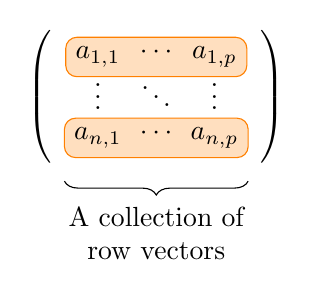
\begin{tikzpicture}[baseline=(m-2-1.base)]
        \matrix [matrix of math nodes,left delimiter=(,right delimiter=),
        ampersand replacement=\&] (m)
        {
            a_{1,1} \& \cdots \& a_{1,p} \\[-1.5ex]               
            \vdots \& \ddots \& \vdots \\               
            a_{n,1} \& \cdots \& a_{n,p} \\           
        };  
        \begin{scope}[on background layer]
        \draw[color=orange, fill = orange, fill opacity = 0.25, rounded corners] (m-1-1.north west) -- (m-1-3.north east) -- (m-1-3.south east) -- (m-1-1.south west) -- cycle;
        \draw[color=orange, fill = orange, fill opacity = 0.25, rounded corners] (m-3-1.north west) -- (m-3-3.north east) -- (m-3-3.south east) -- (m-3-1.south west) -- cycle;
        \end{scope}
        \draw [decorate, decoration = {brace, amplitude = 5pt, mirror, raise = 3mm}, black] (m-3-1.south west) -- (m-3-3.south east) node[midway, yshift = -2.75em, align = center]{A collection of\\row vectors};
\end{tikzpicture}
=
\begin{tikzpicture}[baseline=(m-2-1.base)]
        \matrix [matrix of math nodes,left delimiter=(,right delimiter=),
        ampersand replacement=\&] (m)
        {
            a_{1,1} \& \cdots \& a_{1,p} \\[-1.5ex]               
            \vdots \& \ddots \& \vdots \\               
            a_{n,1} \& \cdots \& a_{n,p} \\           
        };  
        \begin{scope}[on background layer]
        \draw[color=SteelBlue3, fill = SteelBlue3, fill opacity = 0.25, rounded corners] (m-1-1.north west) -- (m-1-1.north east) -- (m-3-1.south east) -- (m-3-1.south west) -- cycle;
        \draw[color=SteelBlue3, fill = SteelBlue3, fill opacity = 0.25, rounded corners] (m-1-3.north west) -- (m-1-3.north east) -- (m-3-3.south east) -- (m-3-3.south west) -- cycle;
        \end{scope}
        \draw [decorate, decoration = {brace, amplitude = 5pt, mirror, raise = 3mm}, black] (m-3-1.south west) -- (m-3-3.south east) node[midway, yshift = -2.75em, align = center]{A collection of\\column vectors};
\end{tikzpicture}
\end{align}
%https://tex.stackexchange.com/questions/40028/highlight-elements-in-the-matrix

As a result, one additional way to notate a matrix is by writing a matrix as a row vector, where each entry in the vector is a column vector (i.e. a vector of vectors). This is given by 
\begin{align}
    \label{matrixvectornotation}
    \mathbf{A} = \begin{pmatrix}
        \mathbf{a}_1 & \cdots & \mathbf{a}_p
    \end{pmatrix},
\end{align}
where $\mathbf{a}_i$ is the $i^{\text{th}}$ column vector of $\mathbf{A}$. 



\subsection{Matrix (and Vector) Addition and Scalar Multiplication}

Given two matrices $\mathbf{A}_{n \times p}$ and $\mathbf{B}_{n \times p}$, we can perform \mydef{matrix addition} on them to get a new matrix, generally denoted as $\mathbf{A} + \mathbf{B}$. This operation is defined by its elements and is given by 
\begin{align}
    \label{matrixaddition}
    (a+b)_{i,j} = a_{i,j} + b_{i,j},
\end{align}
for all $i \in \{ 1,\ldots,n \}$ and $j \in \{ i,\ldots,p \}$. In other words, to get the $(i,j)^{\text{th}}$ element of $\mathbf{A} + \mathbf{B}$, just add together the $(i,j)^{\text{th}}$ elements of $\mathbf{A}$ and $\mathbf{B}$. 

Another basic operation is \mydef{scalar multiplication}, where a matrix is multiplied by some real number $c$. Denoted as $c \mathbf{A}$, this operation is again defined by its elements and is given by 
\begin{align}
    \label{scalarmultiplication}
    (c a)_{i,j} = c \cdot a_{i,j}.
\end{align}
In other words, to get the $(i,j)^{\text{th}}$ element of $c \mathbf{A}$, just multiply the $(i,j)^{\text{th}}$ element of $\mathbf{A}$ by $c$.

These operations are the same for vectors (remember that we are treating them as essentially the same type of object). That is, given two vectors $\mathbf{v} = (v_1, \ldots, v_n)$ and $\mathbf{w} = (w_1,\ldots,w_n)$, we have $\mathbf{v} + \mathbf{w} = (v_1 + w_1, \ldots, v_n + w_n)$ and $c \mathbf{v} = (cv_1, \ldots, cv_n)$.





\subsection{Matrix (and Vector) Multiplication}

Keeping in mind that we will be treating vectors as $n \times 1$ matrices, we will now introduce the idea of multiplying two matrices together. \mydef{Matrix Multiplication} between two matrices $\mathbf{A}_{n \times p}$ and $\mathbf{B}_{p \times q}$ gives us a third matrix, denoted as $\mathbf{AB}$, and is defined by its elements as 
\begin{align}
\label{mmult}
    (ab)_{i,j} = \sum_{k=1}^p a_{i,k} b_{k,j}.
\end{align}
This formula can be somewhat daunting at first glance, and there are several subtleties that need to be understood. First, we can see that in order for this operation to be defined, the number of \textit{columns} of $\mathbf{A}$ must equal the number of \textit{rows} of $\mathbf{B}$. As a result, the new matrix $\mathbf{AB}$ has $n$ rows and $q$ columns; that is, it has the same number of rows as $\mathbf{A}$ and the same number of columns as $\mathbf{B}$. (\ref{mmult}) gives us a systematic way to compute each element of $\mathbf{AB}$ by using the rows of $\mathbf{A}$ and the columns of $\mathbf{B}$, but this process is rather tedious, and computer software such as \texttt{R} or \texttt{MATLAB} can be used to easy multiply matrices.

%(\ref{mmult}) gives us a systematic way to compute each element of $\mathbf{C}$ by using the rows of $\mathbf{A}$ and the columns of $\mathbf{B}$ (assuming that $\mathbf{A}$ has $p$ columns and $\mathbf{B}$ has $p$ rows:
%\begin{enumerate}
%    \item To find $c_{i,j}$, i.e. the element in $\mathbf{C}$ in the $i^{\text{th}}$ row and the $j^{\text{{th}}}$ column, look at the $i^{\text{th}}$ row of $\mathbf{A}$ and the $j^{\text{th}}$ row of $\mathbf{B}$.
%    \item Take the first element in the $i^{\text{th}}$ row of $\mathbf{A}$, $a_{i,1}$, and multiply it by the first element in the $j^{\text{th}}$ row of $\mathbf{B}$, $b_{1,j}$. You end up with $a_{i,1} b_{1,j}$.
%    \item Repeat this step again for the second element of each respective vector; you will end up with $a_{i,2} b_{2,j}$.
%    \item Repeat this process up until the last element, which will occur after $p$ iterations (since there are $p$ elements in each row vector of $\mathbf{A}$ and $p$ elements in each column vector of $\mathbf{B}$).
%    \item At this point you will have $p$ numbers, given by $\{ a_{i,1}b_{1,j},\ldots, a_{i,p}b_{p,j}\}$. Add up all of these numbers to get $c_{i,j}$.
%    \item Repeat this process for all $i \in \{ 1,\ldots,n \}$ and $j \in \{ 1,\ldots,q \}$. You will have to do this process $nq$ times.
%\end{enumerate}

\subsection{Some Special Vectors and Matrices}

We have already spend a good deal of time talking about the transpose. However, there are several other special vectors and matrices that we should become familiar with before going forward.

\subsubsection{The Null Vector and the Ones Vector}

The \mydef{null vector}, denoted as $\mathbf{0}$, is simply an $n$-vector where \textit{every} element is equal to 0. In other words, $\mathbf{0} = (0,\ldots,0)$. Similarly, the \mydef{ones vector}, denoted as $\mathbf{1}$, is an $n$-vector where every element is equal to 1. In other words, $\mathbf{1} = (1,\ldots,1)$.

\subsubsection{The Transpose}

For an $n \times p$ matrix $\mathbf{A}$, its \mydef{transpose}, denoted as $\mathbf{A}^T$, is defined as 
\begin{align}
    \label{transpose}
    \mathbf{A}^T = (a^T_{i,j}) = (a_{j,i}),
\end{align}
for $i \in \{ 1,\ldots,n \}$ and $j \in \{ 1,\ldots,p \}$. In other words, we take the rows of $\mathbf{A}$ and re-write them as the columns of $\mathbf{A}^T$. Note that we are using the $a^T_{i,j}$ to denote the $(i,j)^{\text{th}}$ element of $\mathbf{A}^T$. If we want to explicitly look at the elements of $\mathbf{A}^T$, then the transpose of (\ref{eq4}) can be written as
\begin{align}
    \label{transposefull}
    \mathbf{A}^T = \begin{pmatrix}
        a_{1,1} & \cdots & a_{p,1} \\
        \vdots & \ddots & \vdots \\
        a_{1,n} & \cdots & a_{n,p}
    \end{pmatrix}.
\end{align}

%More properties about the transpose will be further explored after matrix multiplication is defined. 

We should note the relationship between the transpose and vectors. Namely, the transpose of a column vector (\ref{eq4}) is a row vector (\ref{rv1}), and similarly, the transpose of a row vector is a column vector. 

Similar to (\ref{matrixvectornotation}), we can represent $\mathbf{A}$ as a vector. Only this time, we will represent it as a column vector, where the $i^{\text{th}}$ entry is the transpose of the $i^{\text{th}}$ column vector of $\mathbf{A}$, which is a row vector. This notation is given by 
\begin{align}
    \label{transposevectornotation}
    \mathbf{A}^T = \begin{pmatrix}
        \mathbf{a}_1^T \\ \vdots \\ \mathbf{a}_p^T
    \end{pmatrix},
\end{align}
where $\mathbf{a}_i$ is the $i^{\text{th}}$ column vector of $\mathbf{A}$.

%Now that matrix multiplication is defined, we are ready to show some more properties. In order to show that two matrices are equivalent, we must show that the $(i,j)^{\text{th}}$ element of the first matrix is equal to the $(i,j)^{\text{th}}$ element of the second matrix. 
%Before we start, I want to mention that these proofs are fairly non-intuitive, as they only involve carefully applying the definition of the transpose, (\ref{transpose}), to various different elements of matrices. 

%\textbf{Property 1}: For any matrix $\mathbf{A}_{n \times p}$, we have $(\mathbf{A}^T)^T = \mathbf{A}$. That is, taking the transpose of the transpose returns the original matrix. This is easy to see; recall from (\ref{transpose}) that $a^T_{i,j} = a_{j,i}$. Then applying the transpose again gives us $(a^T)^T_{i,j} = a^T_{j,i} = a_{i,j}$, which shows that $(\mathbf{A}^T)^T = \mathbf{A}$. \done

%\textbf{Property 2}: For any two matrices $\mathbf{A}_{n \times p}$ and $\mathbf{B}_{n \times p}$, we have $(\mathbf{A} + \mathbf{B})^T = \mathbf{A}^T + \mathbf{B}^T$. In other words, in order to find the transpose of the sum of two matrices, you can instead first find the transpose of each matrix on its own and then add them together. This proof is also fairly straightforward; recall that each element of $\mathbf{A} + \mathbf{B}$ is given by $(a+b)_{i,j} = a_{i,j} + b_{i,j}$. Then applying the transpose to this gives us 
%\begin{align*}
%    (a+b)^T_{i,j} = (a+b)_{j,i} = a_{j,i} + b_{j,i} = a^T_{i,j} + b^T_{i,j},
%\end{align*}
%which shows that $(\mathbf{A} + \mathbf{B})^T = \mathbf{A}^T + \mathbf{B}^T$. \done 

The transpose has several useful properties that we will take advantage of when working with the SVD. To start, we will show that for any matrix $\mathbf{A}_{n \times p}$, we have $(\mathbf{A}^T)^T = \mathbf{A}$. That is, taking the transpose of the transpose returns the original matrix. This is easy to see; recall from (\ref{transpose}) that $a^T_{i,j} = a_{j,i}$. Then applying the transpose again gives us $(a^T)^T_{i,j} = a^T_{j,i} = a_{i,j}$, which shows that $(\mathbf{A}^T)^T = \mathbf{A}$. \done

Next we will show that for two matrices $\mathbf{A}_{n \times p}$ and $\mathbf{B}_{p \times q}$, we have $(\mathbf{AB})^T = \mathbf{B}^T \mathbf{A}^T$. We will prove this by showing that the $(i,j)^{\text{th}}$ element of $(\mathbf{AB})^T$ and $\mathbf{B}^T \mathbf{A}^T$ are equal; that is, $(ab)^T_{i,j} = (b^T a^T)_{i,j}$ for all $i \in \{ 1,\ldots,n \}$ and $j \in \{ 1,\ldots,q \}$.
Recall from (\ref{mmult}) that the elements of the product of two matrices are given by 
\begin{align*}
    (ab)_{i,j} = \sum_{k=1}^p a_{i,k} b_{k,j}.
\end{align*}
Then applying the transpose to this gives us 
\begin{align*}
    (ab)^T_{i,j} = (ab)_{j,i} = \sum_{k=1}^p a_{j,k} b_{k,i} = \sum_{k=1}^p b^T_{i,k} a^T_{k,j} = (b^T a^T)_{i,j},
\end{align*}
which shows that $(\mathbf{AB})^T = \mathbf{B}^T \mathbf{A}^T$. \done 

\subsubsection{Symmetric Matrices}

A matrix $\mathbf{A}$ is \mydef{symmetric} if it is equal to its transpose, i.e. $\mathbf{A} = \mathbf{A}^T$. That is, $a_{i,j} = a_{j,i}$ for all $i \in \{ 1, \ldots, n\}$ and $j \in \{ 1,\ldots,p \}$. Note that in order for a matrix to be symmetric, it must be square. There are some important properties that symmetric matrices have, but we will show them later on when orthogonal matrices and eigenvectors are introduced. 

\subsubsection{The Main Diagonal and Diagonal Matrices}

The \mydef{main diagonal} of a matrix $\mathbf{A}$, denoted as $\mathrm{diag}(\mathbf{A})$, is the collection of elements $a_{i,j}$ such that $i=j$, that is, all elements of the form $a_{i,i}$. For a matrix $\mathbf{A}_{n \times p}$, we have \begin{align}
    \label{diagonal}
    \mathrm{diag}(\mathbf{A}) = \big\{ a_{1,1}, \ldots, a_{\min\{n,p\},\min\{n,p\}} \big\}.
\end{align}
The notation of $\min\{n,p\}$ may be slighlty confusing, but all it means is that the maximum amount of elements that can be on the main diagonal of a matrix is the smaller amount between $n$ and $p$. To illustrate this, the main diagonal of matrices $\mathbf{A}$, $\mathbf{B}$, and $\mathbf{C}$ are highlighted below in orange. We have three separate cases:
\begin{enumerate}
    \item $\mathbf{A}_{n \times n}$ is a square matrix.
    \item $\mathbf{B}_{n \times p}$ is a matrix such that $n>p$. That is, the matrix has more rows than columns. 
    \item $\mathbf{C}_{n \times p}$ is a matrix such that $n<p$. That is, the matrix has more columns than rows. 
\end{enumerate}

\begin{align*}
 \mathbf{A} =
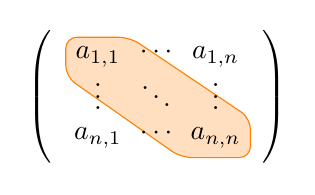
\begin{tikzpicture}[baseline=(m-2-1.base)]
        \matrix [matrix of math nodes,left delimiter=(,right delimiter=),
        ampersand replacement=\&] (m)
        {
            a_{1,1} \& \cdots \& a_{1,n} \\[-1.5ex]               
            \vdots \& \ddots \& \vdots \\               
            a_{n,1} \& \cdots \& a_{n,n} \\           
        };  
        \begin{scope}[on background layer]
        \draw[color=orange, fill = orange, fill opacity = 0.25, rounded corners] (m-1-1.north west) -- (m-1-1.north east) -- (m-3-3.north east) -- (m-3-3.south east) -- (m-3-3.south west) -- (m-1-1.south west) -- cycle;
        \end{scope}
\end{tikzpicture},
 ~~~~\mathbf{B} =
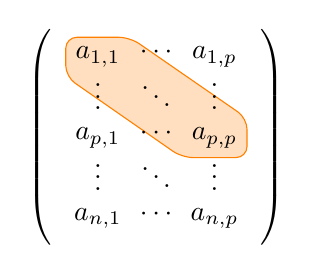
\begin{tikzpicture}[baseline=(m-3-1.base)]
        \matrix [matrix of math nodes,left delimiter=(,right delimiter=),
        ampersand replacement=\&] (m)
        {
            a_{1,1} \& \cdots \& a_{1,p} \\[-1.5ex]               
            \vdots \& \ddots \& \vdots \\               
            a_{p,1} \& \cdots \& a_{p,p} \\[-1.5ex]  
            \vdots \& \ddots \& \vdots \\               
            a_{n,1} \& \cdots \& a_{n,p} \\
        };  
        \begin{scope}[on background layer]
        \draw[color=orange, fill = orange, fill opacity = 0.25, rounded corners] (m-1-1.north west) -- (m-1-1.north east) -- (m-3-3.north east) -- (m-3-3.south east) -- (m-3-3.south west) -- (m-1-1.south west) -- cycle;
        \end{scope}
\end{tikzpicture},
~~~~\mathbf{C} =
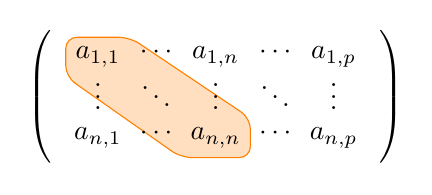
\begin{tikzpicture}[baseline=(m-2-1.base)]
        \matrix [matrix of math nodes,left delimiter=(,right delimiter=),
        ampersand replacement=\&] (m)
        {
            a_{1,1} \& \cdots \& a_{1,n} \& \cdots \& a_{1,p} \\[-1.5ex]               
            \vdots \& \ddots \& \vdots \& \ddots \& \vdots \\
            a_{n,1} \& \cdots \& a_{n,n} \& \cdots \& a_{n,p}\\
        };  
        \begin{scope}[on background layer]
        \draw[color=orange, fill = orange, fill opacity = 0.25, rounded corners] (m-1-1.north west) -- (m-1-1.north east) -- (m-3-3.north east) -- (m-3-3.south east) -- (m-3-3.south west) -- (m-1-1.south west) -- cycle;
        \end{scope}
\end{tikzpicture}
\end{align*}
We can see that if $n>p$ (more rows than columns), then the maximum number of elements in $\mathrm{diag}(\mathbf{A})$ is $p$, and if $n<p$ (more columns than rows), then the maximum number of elements in $\mathrm{diag}(\mathbf{A})$ is $n$.

A \mydef{diagonal matrix}, generally denoted as $\mathbf{D}$, is a matrix whose only non-zero entries are elements along its main diagonal. That is, $d_{i,j} = 0 \text{ if } i \not = j$. 

When you multiply a diagonal matrix by itself, $\mathbf{D}^2$, the diagonal of the resulting matrix has the squared values of the original matrix, and zeros in every other entry. That is, $\mathbf{D}^2$ is also diagonal, and 
\begin{align}
    \label{squarediagonal}
    (d^2)_{i,j} = \begin{cases}
        (d_{i,i})^2 & \text{if } i = j \\
        0 & \text{if } i \not = j
    \end{cases}.
\end{align}
This is easy to see using (\ref{mmult}), as the elements of $\mathbf{D}^2$ are given by 
\begin{align*}
    (d^2)_{i,j} \sum_{k=1}^n d_{i,k} d_{k,j} = d_{i,i} d_{i,j} +  \sum_{\substack{k=1\\k\not=i}}^n d_{i,k} d_{k,j} = d_{i,i} d_{i,j}.
\end{align*}
If $i=j$, then $(d^2)_{i,j} = (d_{i,i})^2$, but if $i \not = j$, then $(d^2)_{i,j} = d_{i,i} \cdot 0 = 0$, which shows (\ref{squarediagonal}).

One other thing to note is that all diagonal matrices are symmetric. That is, for a diagonal matrix $\mathbf{D}$, we have $\mathbf{D} = \mathbf{D}^T$.

\subsubsection{The Identity Matrix}

A special case of the diagonal matrix is the \mydef{identity matrix}, denoted as $\mathbf{I}$, is a square diagonal matrix whose elements along the diagonal are all equal to 1. That is,
\begin{align}
    \label{identity}
    \iota_{i,j} = \begin{cases}
        1, & \text{if } i = j \\
        0, & \text{if } i \not = j
    \end{cases},
\end{align}
and $\mathrm{diag}(\mathbf{I}) = \{ 1,\ldots,1 \}$. It is important to stress that, unlike other diagonal matrices, the identity matrix must be square. 

The identity matrix is named the way it is because of the fact that multiplying any matrix $\mathbf{A}_{n \times p}$ by it returns $\mathbf{A}$. In other words, 
\begin{align}
    \mathbf{I}_{n \times n} \mathbf{A}_{n \times p} = \mathbf{A}_{n \times p} \mathbf{I}_{p \times p} = \mathbf{A}_{n \times p}.
\end{align}
This is easy to see using (\ref{mmult}) and (\ref{identity}), since
\begin{align*}
    (\iota a)_{i,j} = \sum_{k=1}^n \iota_{i,k} a_{k,j} = \iota_{i,i} a_{i,j} + \sum_{\substack{k=1\\k\not=i}}^n \iota_{i,k} a_{k,j} = a_{i,j}
\end{align*}
and 
\begin{align*}
    (a\iota)_{i,j} = \sum_{k=1}^p a_{i,p} \iota_{p,j} = a_{i,j} \iota_{j,j} + \sum_{\substack{k=1\\k\not=j}}^p \iota_{i,k} a_{k,j} = a_{i,j}.
\end{align*}

\subsubsection{Matrix Inversion}

Given a square matrix $\mathbf{A}_{n \times n}$, its \mydef{inverse}, denoted as $\mathbf{A}^{-1}$, is defined as the matrix such that 
\begin{align}
    \label{inverse}
    \mathbf{A} \mathbf{A}^{-1} = \mathbf{A}^{-1} \mathbf{A} = \mathbf{I}.
\end{align}
In other words, if you multiply a matrix by its inverse, you get the identity matrix.

Note that we mentioned the matrix $\mathbf{A}$ must be square in order to be inverted. This technically is not entirely true, since a non-square matrix can have a \mydef{left inverse} and a \mydef{right inverse}. However, for the purposes of SVD, the only matrices we will be inverting will be square, so we will not worry about this. 

In general, computing the inverse of a matrix by hand is difficult, and no formulas to do so will be presented here; any software program such as \texttt{R} or \texttt{MATLAB} can compute the inverse. For the purposes of SVD, some inverse matrices will be of interest to us. However, those will be orthogonal matrices (to be covered soon), which are easy to take the inverse of. 

\subsubsection{Inner Products, Norms, Orthogonal Vectors, and Unit Vectors}

For two vectors $\mathbf{v} = (v_1,\ldots,v_n)$ and $\mathbf{w}=(w_i,\ldots,w_n$, both of order $n$, the \mydef{inner product} between them, denoted by $\langle \mathbf{v}, \mathbf{w} \rangle$, is defined as 
\begin{align}
    \label{inprod}
    \langle \mathbf{v}, \mathbf{w} \rangle = \mathbf{v}^T \mathbf{w} = \sum_{i = 1}^n v_i w_i
\end{align}
The inner product is also commonly referred to as the \mydef{dot product} and denoted $\mathbf{v} \cdot \mathbf{w}$, but we avoid that notation here. One thing to note that inner products are commutative, since 
\begin{align*}
    \langle \mathbf{v}, \mathbf{w} \rangle = \mathbf{v}^T \mathbf{w} = \sum_{i = 1}^n v_i w_i = \sum_{i = 1}^n w_i v_i  = \mathbf{w}^T \mathbf{v} = \langle \mathbf{w}, \mathbf{v} \rangle.
\end{align*}

We are so interested in the inner product of two vectors since it gives us a method to determine whether or not the vectors are \mydef{orthogonal}. Two vectors are orthogonal if they are \mydef{perpendicular}, which is true if 
\begin{align}
    \label{orthogonal}
    \langle \mathbf{v},\mathbf{w} \rangle = 0.
\end{align}
%Given the brevity of this review, we have not described the geometric intuition of vectors, and so the idea of two vectors being ``parallel" may seem nonsensical. 
%Just know that there is a very strong and rewarding geometric intuition to these ideas, and those interested can find many more in-depth sources.

For a vector $\mathbf{v} = (v_1,\ldots,v_n)$, the \mydef{Euclidean norm}, or \mydef{$\ell_2$-norm}, notated as $\| \mathbf{v} \|$, is defined as 
\begin{align}
    \label{eucnorm}
    \| \mathbf{v} \| = \sqrt{\langle \mathbf{v}, \mathbf{v} \rangle} = \sqrt{\sum_{i = 1}^n v_i^2}.
    %\left( \sum_{i = 1}^n v_i^2 \right)^{1/2}.
\end{align}
That is, to calculate the $\ell_2$-norm of a vector $\mathbf{v}$, we simply take the square root of the inner product of the vector with itself. The reader should note, then, that $\| \mathbf{v} \|^2 = \mathbf{v}^T \mathbf{v} = \langle \mathbf{v},\mathbf{v} \rangle$.

The $\ell_2$-norm is used to measure the ``length'' of a vector. The reason we are so interested in the $\ell_2$-norm is because it provides us a method to generate a \mydef{unit vector}, which is a vector with length 1 (i.e. an $\ell_2$-norm equal to 1). Given a vector $\mathbf{v} = (v_1,\ldots,v_n)$, it is easy to construct a corresponding unit vector, denoted as $\mathbf{u} = (u_1,\ldots,u_n)$, by dividing $\mathbf{v}$ by $\| \mathbf{v} \|$; that is, 
\begin{align}
    \label{unitvector}
    \mathbf{u} = \frac{\mathbf{v}}{\| \mathbf{v} \|}.
\end{align}
In other words, each element of $\mathbf{u}$ is just each element of $\mathbf{v}$ divided by $\| \mathbf{v} \|$, i.e. $u_i = v_i / \| \mathbf{v} \|$ for $i \in \{ 1,\ldots,n \}$.

%Looking at (\ref{inpasmul}) and (\ref{eucnorm}), we can see that 
%\begin{align}
%    \label{normprodrel}
%    \langle \mathbf{v}, \mathbf{v} \rangle = \mathbf{v}^T \mathbf{v} = \| \mathbf{v} \|^2.
%\end{align}

Finally, two vectors $\mathbf{v}$ and $\mathbf{w}$ are \mydef{orthonormal} if they are orthogonal and both unit vectors. That is, if $\langle \mathbf{v},\mathbf{w} \rangle = 0$ and $\| \mathbf{v} \| = \| \mathbf{w} \| = 1$, then $\mathbf{v}$ and $\mathbf{w}$ are orthonormal. 

\subsubsection{Outer Products}

Given two $n$-vectors $\mathbf{v}$ and $\mathbf{w}$, their outer product, denoted as $\mathbf{v} \otimes \mathbf{w}$, is defined as 
\begin{align}
    \label{outerproduct}
    \mathbf{v} \otimes \mathbf{w} = \mathbf{v} \mathbf{w}^T.
\end{align}
Note the similarity to the inner product (\ref{inprod}). Given the dimensions of $\mathbf{v}$ ($n \times 1$) and $\mathbf{w}^T$ ($1 \times n$), the outer product will result in a square matrix, whose elements are given by 
\begin{align}
    (v \otimes w)_{i,j} = v_i w_j.
\end{align}

\subsubsection{Orthogonal Matrices}

An \mydef{orthogonal matrix}, generally denoted as $\mathbf{U}$, is a matrix whose row vectors and column vectors make up a set of mutually orthonormal (\textit{not} orthogonal) vectors. That is, for $\mathbf{U}$ to be orthogonal, all of its row vectors must be orthonormal to each other and all of its column vectors must be orthonormal to each other. While a non-square matrix may possibly be orthogonal, there are some subtle technicalities that we will not pursue further, and from now on we will assume that orthogonal matrices are square.

One useful property about orthogonal matrices is that their inverse is given by their transpose. That is, for an orthogonal matrix $\mathbf{U}_{n \times n}$, we have $\mathbf{U}^{-1} = \mathbf{U}^T$. This property is extremely helpful because it makes determining the inverse very easy.

To do this, we will show that $\mathbf{U}^T \mathbf{U} = \mathbf{I}$. We will first use (\ref{matrixvectornotation}) and (\ref{transposevectornotation}) two write this product as a product of vectors, so 
\begin{align*}
    \mathbf{U}^T \mathbf{U} = \begin{pmatrix}
        \mathbf{u}_1^T \\ \vdots \\ \mathbf{u}_n^T
    \end{pmatrix} 
    \begin{pmatrix}
        \mathbf{u}_1 & \cdots & \mathbf{u}_n
    \end{pmatrix},
\end{align*}
where $\mathbf{u}_i$ is the $i^{\text{th}}$ column vector of $\mathbf{U}$. The elements of this product, which is an outer product, are given by 
\begin{align*}
    (u^T u)_{i,j} = \mathbf{u}_i^T \mathbf{u}_j.
\end{align*}
We will now take advantage of the fact that the vectors are orthonormal. For any two of the vectors $\mathbf{u}_i$ and $\mathbf{u}_j$, we have $\mathbf{u}_i^T \mathbf{u}_j = \langle \mathbf{u}_i, \mathbf{u}_j \rangle = 0$, since they are orthogonal. We also have $\mathbf{u}_i^T \mathbf{u}_i = \| \mathbf{u}_i \|^2 = 1$, since they are unit vectors. Then from this, we have 
\begin{align*}
    (u^T u)_{i,j} = \begin{cases}
        1, & \text{if } i = j \\
        0, & \text{if } i \not = j
    \end{cases}.
\end{align*}
These are the same elements as the identity matrix (\ref{identity}), which shows that $\mathbf{U}^T \mathbf{U} = \mathbf{I}$. Finally, multiply both sides of this equation by $\mathbf{U}^{-1}$, and we have $\mathbf{U}^T = \mathbf{U}^{-1}$. That is, for an orthogonal matrix, its inverse is its transpose. \done

\subsubsection{Gramian Matrices}

Given a matrix $\mathbf{A}_{n \times p}$, its two corresponding \mydef{Gramian matrices} are given by $\mathbf{A} \mathbf{A}^T$ and $\mathbf{A}^T \mathbf{A}$. From now on we will refer to the matrix $\mathbf{A} \mathbf{A}^T$ as the \mydef{left Gramian matrix} and $\mathbf{A}^T \mathbf{A}$ as the \mydef{right Gramian matrix}.

One useful property of the Gramian matrices are that they are always symmetric. This is easy to see, since 
\begin{align*}
    (\mathbf{A} \mathbf{A}^T)^T = (\mathbf{A}^T)^T \mathbf{A}^T = \mathbf{A} \mathbf{A}^T
\end{align*}
and 
\begin{align*}
    (\mathbf{A}^T \mathbf{A})^T = \mathbf{A}^T (\mathbf{A}^T)^T = \mathbf{A}^T \mathbf{A}.
\end{align*}

For a right Gramian matrix, we can look at the $(i,j)^{\text{th}}$ element as an inner product as the $i^{\text{th}}$ and $j^{\text{th}}$ column vectors of $\mathbf{A}$. We have 
\begin{align*}
    \mathbf{A}^T \mathbf{A} = \begin{pmatrix}
        \mathbf{a}_1^T \\ \vdots \\ \mathbf{a}_n^T
    \end{pmatrix} 
    \begin{pmatrix}
        \mathbf{a}_1 & \cdots & \mathbf{a}_n
    \end{pmatrix},
\end{align*}
where $\mathbf{a}_i$ is the $i^{\text{th}}$ column vector of $\mathbf{A}$. The elements of this outer product are then given by 
\begin{align}
    \label{rightgramianelements}
    (a^T a)_{i,j} = \mathbf{a}_i^T \mathbf{a}_j.
\end{align}
Since the inner product is commutative, we have $(a^T a)_{i,j} = (a^T a)_{j,i} = (a^T a)_{i,j}^T$, which is another indication that the right Gramian matrix is symmetric. 

\subsection{Eigenvalues and Eigenvectors}

Given a \textit{square} matrix $\mathbf{A}_{n \times n}$, the non-zero vector $\mathbf{v}$ is an \mydef{eigenvector} of $\mathbf{A}$ if it satisfies the equation 
\begin{align}
    \label{eigenvector}
    \mathbf{A} \mathbf{v} = \lambda \mathbf{v},
\end{align}
where we say the scalar $\lambda$ is the corresponding \mydef{eigenvalue}. What this means is that if we multiply a matrix $\mathbf{A}$ by an eigenvector $\mathbf{v}$, the resulting vector is the same as just taking the original eigenvector and scaling it up by a factor of $\lambda$. 

To solve for the eigenvectors and their corresponding eigenvalues, we will first determine the eigenvalues. To start, we can see that $\lambda \mathbf{v} = \lambda \mathbf{Iv}$, since multiplying any vector or matrix by the identity matrix does not change its value. Next, subtract this from both sides of the equation, which gives us $\mathbf{Av} - \lambda \mathbf{Iv} = \mathbf{0}$, where $\mathbf{0}$ is the null vector. Finally factor out $\mathbf{v}$ to get 
\begin{align}
    \label{alteigenvalue}
    (\mathbf{A} - \lambda \mathbf{I}) \mathbf{v} = \mathbf{0}.
\end{align}
Since we required $\mathbf{v} \not = \mathbf{0}$, the only way that (\ref{alteigenvalue}) holds is for $\mathrm{det} (\mathbf{A} - \lambda \mathbf{I}) = 0$, where $\mathrm{det}(\cdot)$ is the \mydef{determinant}. In this review we did not discuss matrix inversion, so the reasoning as to why the determinant must equal 0 will be unclear to some. 

The importance of (\ref{eigenvector}) for understanding SVD cannot be understated, as there is a strong connection between eigenvalues/eigenvectors and singular values/singular vectors. 

Some of the special matrices mentioned in Section 2.4 have very useful properties. The first we would like to examine is that for a symmetric matrix $\mathbf{A}$, the eigenvectors corresponding to \textit{different} eigenvalues 
%(e.g. eigenvectors $\mathbf{v}_1$ and $\mathbf{v}_2$ with corresponding eigenvalues $\lambda_1$ and $\lambda_2$ such that $\lambda_1 \not = \lambda_2$)
\textit{will always be orthogonal}. 
To see this, let $\mathbf{v}_i$ and $\mathbf{v}_j$ be the $i^{\text{th}}$ and $j^{\text{th}}$ eigenvectors of a symmetric matrix $\mathbf{A}_{n \times p}$ with corresponding eigenvalues $\lambda_i$ and $\lambda_j$, and assume that $\lambda_i \not = \lambda_j$. We can see that 
\begin{align*}
    \lambda_i \langle \mathbf{v}_i, \mathbf{v}_j \rangle = \lambda_i \mathbf{v}_i^T \mathbf{v}_j = (\lambda_i \mathbf{v}_i)^T \mathbf{v}_j = (\mathbf{A} \mathbf{v}_i)^T \mathbf{v}_j = \mathbf{v}_i^T \mathbf{A}^T \mathbf{v}_j = \mathbf{v}_i^T (\mathbf{A}^T \mathbf{v}_j)
\end{align*}
where we used (\ref{eigenvector}). Now, since $\mathbf{A}$ is symmetric, we have $\mathbf{A} = \mathbf{A}^T$, and so our equation becomes 
\begin{align*}
    \mathbf{v}_i^T (\mathbf{A}^T \mathbf{v}_j) = \mathbf{v}_i^T (\mathbf{A} \mathbf{v}_j) = \mathbf{v}_i^T (\lambda_j \mathbf{v}_j) = \lambda_j \mathbf{v}_i^T \mathbf{v}_j = \lambda_j \langle \mathbf{v}_i, \mathbf{v}_j \rangle,
\end{align*}
and this shows that $\lambda_j \langle \mathbf{v}_i, \mathbf{v}_j \rangle = \lambda_j \langle \mathbf{v}_i, \mathbf{v}_j \rangle$. We can re-arrange this to get $(\lambda_i - \lambda_j) \langle \mathbf{v}_i, \mathbf{v}_j \rangle = 0$, and since $\lambda_i \not = \lambda_j$, we have $\lambda_i - \lambda_j \not = 0$, and so $\langle \mathbf{v}_i, \mathbf{v}_j \rangle = 0$, making the two eigenvectors orthogonal. \done 

%http://www-users.math.umn.edu/~olver/num_/lnv.pdf
%http://mlwiki.org/index.php/Eigendecomposition




%singular values
%https://math.stackexchange.com/questions/2103056/proof-of-left-and-right-singular-vector-in-svd

\section{The Singular Value Decomposition}

\subsection{Singular Values and Singular Vectors}

For a given matrix $\mathbf{A}_{n \times p}$, a non-negative scalar $\sigma$ is a \mydef{singular value}, with a corresponding \mydef{left singular vector} $\mathbf{u}$ and \mydef{right singular vector} $\mathbf{v}$ if they satisfy the two equations 
\begin{align}
    \label{singularvalues}
    \begin{split}
        \mathbf{A} \mathbf{v} &= \sigma \mathbf{u} \\
        \mathbf{A}^T \mathbf{u} &= \sigma \mathbf{v}.
    \end{split}
\end{align}



\section{Application to Statistics and Data Science}

Now that the theory of SVD has been introduced, we will now examine \textit{how} it is used for applications in statistics and data analysis. 

\subsection{Preliminary Information}

\subsubsection{The Data Matrix}

For a sample of collected data, several \mydef{observations} (also called \mydef{data points}) are made, where data is collected for each one. For each observation, there are several  \mydef{predictors} (also known as \mydef{features} or \mydef{variables}) that are recorded for each one. In general, there will be $n$ observations and $p$ predictors, and we will let $x_{i,j}$ denote the value of the $j^{\text{th}}$ predictor for the $i^{\text{th}}$ observation. We will be storing out data in a \mydef{data matrix}, denoted as $\mathbf{X}_{n \times p}$, where $x_{i,j}$ is the $(i,j)^{\text{th}}$ entry in the matrix. In other words, 
\begin{align}
    \label{datamatrix}
    \mathbf{X} = \begin{pmatrix}
        x_{1,1} & \cdots & x_{1,p} \\
        \vdots & \ddots & \vdots \\
        x_{n,1} & \cdots & x_{n,p}
    \end{pmatrix}.
\end{align}
The $i^{\text{th}}$ row of $\mathbf{X}$, which we will denote as $\mathbf{n}_i$, can be viewed as the information for the $i^{\text{th}}$ observation, while the $j^{\text{th}}$ column, denoted as $\mathbf{p}_j$, can be viewed as the information for the $j^{\text{th}}$ predictor. As a result, we can also write $\mathbf{X}$ in two different ways:
\begin{enumerate}
    \item As a \textit{row vector} (with $n$ elements), where the $i^{\text{th}}$ element is $\mathbf{p}_i$.
    \item As a \textit{column vector} (with $p$ elements), where the $i^{\text{th}}$ element is $\mathbf{n}_i$.
\end{enumerate}
In other words, 
\begin{align}
    \label{datamatrixasvector}
    \mathbf{X} = \begin{pmatrix}
        \mathbf{p}_1 & \cdots & \mathbf{p}_p
    \end{pmatrix} = \begin{pmatrix}
        \mathbf{n}_1 \\ \vdots \\ \mathbf{n}_n
    \end{pmatrix}.
\end{align}
We will be more interested in the first alternative expression. For notation, if we need to look at the individual elements of $\mathbf{p}_j$, we will write it as $\mathbf{p}_j = (x_{1,j},\ldots,x_{n,j})$. Similarly for $\mathbf{n}_i$, we have $\mathbf{n}_i = (x_{i,1},\ldots,x_{i,p})^T$.

\subsubsection{Covariance and the Covariance Matrix}

Given two predictors $\mathbf{p}_i$ and $\mathbf{p}_j$, it is often of interest to figure out how related they are to each other. One way to do this is to measure how much each predictor varies with each other. In other words, we would like to know how changes in the first variable are related to changes in the second. 

To do this, we will use the \mydef{sample covariance} between the two predictors. Denoted as $\mathrm{Cov}(\mathbf{p}_i, \mathbf{p}_j)$, it is defined as 
\begin{align}
    \label{covariance}
    \mathrm{Cov}(\mathbf{p}_i, \mathbf{p}_j) = \frac{1}{n-1} \sum_{k=1}^n (x_{k,i} - \mu_i)(x_{k,j}-\mu_j).
\end{align}
The use of $n-1$ in the denominator as opposed to $n$ is known as \mydef{Bessel's correction}. The terms $\mu_i$ and $\mu_j$ are the \mydef{sample means} for the two predictors $\mathbf{p}_i$ and $\mathbf{p}_j$, respectively. To calculate the sample mean for a predictor, simply take each element of the predictor and divide by $n$. That is,
\begin{align}
    \label{samplemean}
    \mu_i = \frac{1}{n} \sum_{k=1}^n x_{k,i}.
\end{align}
We can also express (\ref{covariance}) as an inner product between the two predictors. This is given by 
\begin{align}
    \label{covarianceasinnerproduct}
    \mathrm{Cov}(\mathbf{p}_i, \mathbf{p}_j) = \frac{(\mathbf{p}_i - \bm{\mu}_i)^T(\mathbf{p}_j - \bm{\mu}_j)}{n-1} = \frac{\langle \mathbf{p}_i - \bm{\mu}_i, \mathbf{p}_j - \bm{\mu}_j \rangle}{n-1}.
\end{align}
Here, the notation $\bm{\mu}_i$ represents the \mydef{sample mean vector} for $\mathbf{p}_i$, and is given by $\bm{\mu}_i = \mu_i \mathbf{1}$. In other words, $\bm{\mu}_i$ is a vector where every element is $\mu_i$. Note that because inner products are commutative, we have $\mathrm{Cov}(\mathbf{p}_i, \mathbf{p}_j) = \mathrm{Cov}(\mathbf{p}_j, \mathbf{p}_i)$.

A special case of the sample covariance is the \mydef{sample variance} of a predictor, denoted as $\mathrm{Var}(\mathbf{p}_i)$, which is just the covariance between the predictor and \textit{itself}. That is, 
\begin{align}
    \label{variance}
    \mathrm{Var}(\mathbf{p}_i) = \mathrm{Cov}(\mathbf{p}_i, \mathbf{p}_i).
\end{align}

It is often of interest for us to \mydef{center} the data, the process of setting the sample average to zero for each predictor (i.e. $\mu_i = 0$ for all $i \in \{ 1,\ldots,n \}$). To do this, we simply have to take each predictor $\mathbf{p}_{i}$ and subtract $\bm{\mu}_i$. In other words, the \mydef{centered predictors} are given by 
\begin{align}
    \label{centeredpredictors}
    \mathbf{p}_i' = \mathbf{p} - \bm{\mu}_i.
\end{align}
In order to avoid unnecessary notation, and the fact that it is never a computational issue to center the data, \textit{from now on we are going to assume that every data matrix $\mathbf{X}$ is centered, such that $\mu_i = 0$ for all $i \in \{ 1,\ldots,n \}$.} Note that using a centered data matrix as opposed to the original \textit{does not} actually change the covariance.
%; it is really only for notational ease.

Given this, we can re-express (\ref{covariance}) and (\ref{covarianceasinnerproduct}) as 
\begin{align}
    \label{covariancecentered}
    \mathrm{Cov}(\mathbf{p}_i, \mathbf{p}_j) = \frac{1}{n-1} \sum_{k=1}^n x_{k,i}x_{k,j} =  \frac{\mathbf{p}_i^T\mathbf{p}_j}{n-1} = \frac{\langle \mathbf{p}_i, \mathbf{p}_j \rangle}{n-1}.
\end{align}

It will be useful for us to store the covariances between several predictors in a \mydef{covariance matrix}, denoted as $\mathbf{\Sigma}$. The $(i,j)^{\text{th}}$ element of $\mathbf{\Sigma}$, denoted as $\Sigma_{i,j}$, is the covariance between the two predictors $\mathbf{p}_i$ and $\mathbf{p}_j$ (i.e. $\Sigma_{i,j} = \mathrm{Cov}(\mathbf{p}_i, \mathbf{p}_j)$), so
\begin{align}
    \label{covariancematrix}
    \mathbf{\Sigma} = \begin{pmatrix}
        \mathrm{Cov}(\mathbf{p}_1, \mathbf{p}_1) & \cdots & \mathrm{Cov}(\mathbf{p}_1, \mathbf{p}_p) \\
        \vdots & \ddots & \vdots \\
        \mathrm{Cov}(\mathbf{p}_p, \mathbf{p}_1) & \cdots & \mathrm{Cov}(\mathbf{p}_p, \mathbf{p}_p)
    \end{pmatrix}.
\end{align}
We can see that the elements along the main diagonal of $\mathbf{\Sigma}$ are the variances of each of the predictors. Also, since covariance is commutative, we have 
\begin{align*}
    \Sigma_{i,j} = \mathrm{Cov}(\mathbf{p}_i, \mathbf{p}_j) = \mathrm{Cov}(\mathbf{p}_j, \mathbf{p}_i) = \Sigma_{j,i} = \Sigma_{i,j}^T,
\end{align*}
so the covariance matrix is always symmetric. Using (\ref{covariancecentered}), we can re-write the elements of $\mathbf{\Sigma}$ as 
\begin{align*}
    \Sigma_{i,j} = \mathrm{Cov}(\mathbf{p}_i, \mathbf{p}_j) = \frac{\langle \mathbf{p}_i, \mathbf{p}_j \rangle}{n-1} = \frac{\mathbf{p}_i^T\mathbf{p}_j}{n-1}.
\end{align*}
We know that $\mathbf{p}_i^T \mathbf{p}_j$ is the $(i,j)^{\text{th}}$ element of the right Gramian matrix of the data matrix, $\mathbf{X}^T \mathbf{X}$. Therefore, by accounting for the scaling by $1/(n-1)$, we have 
\begin{align}
    \label{covarianceasgramian}
    \mathbf{\Sigma} = \frac{1}{n-1} \mathbf{X}^T \mathbf{X}.
\end{align}
This gives us a very convenient way to calculate the covariance between all $p$ predictors in a data set $\mathbf{X}$ with $n$ observations. 

Eigenvectors $\mathbf{V}$ of the covariance matrix are principal directions. Projections of the data on these eigenvectors are principal components; these projections are given by $\mathbf{US}$.

\end{document}

%eigenvalues and singular values
%https://www.mathworks.com/content/dam/mathworks/mathworks-dot-com/moler/eigs.pdf



%svd and pca
%http://www.ams.org/publicoutreach/feature-column/fcarc-svd

%https://stats.stackexchange.com/questions/2691/making-sense-of-principal-component-analysis-eigenvectors-eigenvalues/140579#140579

%https://stats.stackexchange.com/questions/32174/pca-objective-function-what-is-the-connection-between-maximizing-variance-and-m/136072#136072

%+https://stats.stackexchange.com/questions/134282/relationship-between-svd-and-pca-how-to-use-svd-to-perform-pca?noredirect=1&lq=1

%+https://stats.stackexchange.com/questions/202104/whats-the-physical-meaning-of-the-eigenvectors-of-the-gram-kernel-matrix

%https://stats.stackexchange.com/questions/79043/why-pca-of-data-by-means-of-svd-of-the-data

%https://stats.stackexchange.com/questions/147880/is-pca-still-done-via-the-eigendecomposition-of-the-covariance-matrix-when-dimen

%https://stats.stackexchange.com/questions/192372/relationship-between-eigenvectors-of-frac1nxx-top-and-frac1nx-top

%https://stats.stackexchange.com/questions/189822/how-does-centering-make-a-difference-in-pca-for-svd-and-eigen-decomposition



%quadratic forms
%https://ocw.mit.edu/courses/sloan-school-of-management/15-084j-nonlinear-programming-spring-2004/lecture-notes/lec4_quad_form.pdf

%good stuff on gradients
%https://www.cs.ubc.ca/~schmidtm/Courses/340-F16/linearQuadraticGradients.pdf

%least squares
%http://global.oup.com/booksites/content/0199268010/samplesec3

%lasso
%https://www.cs.ubc.ca/~schmidtm/Documents/2008_Notes_LassoDual.pdf



% section about geometry

\subsubsection{Geometric Intuition of Vectors and Matrices}

There is a strong geometric interpretation for vectors and matrices, and while understanding it may be a little off-course from a basic review, I feel that presenting it here will make understanding Eigendecomposition and the SVD easier. 

An $n$-vector can be thought of as a point in $n$-dimensional space, where each entry of the vector is a coordinate on one of the dimension's axis. Consider a $2$-vector $\mathbf{v} = (v_1,v_2)$; $v_1$ could be thought of as the coordinate along the $x$-axis, while $v_2$ is the coordinate along the $y$-axis. Similarly, a $3$-vector $\mathbf{w} = (w_1,w_2,w_3)$ is a point in $3$-dimensional space. See Figure \ref{vectorfigures} for some examples. 

\begin{figure}
\centering

\begin{tikzpicture}[line width=1pt]

\begin{axis}[
scale=1, %change this to change the size of both images
color= black!50, 
thick,
xmin=-4.9, 
xmax=4.9, 
ymin=-4.9, 
ymax=4.9, 
axis equal image, 
axis lines=middle, 
font=\normalsize,
xtick distance=1,
ytick distance=1,
inner axis line style={stealth-stealth},
xlabel = {$v_1$},
ylabel = {$v_2$},
grid=major,
ticks=none
]

\draw[IndianRed3, thick, -stealth] (0,0) -- (2,3) node[above, text = black] {$(2,3)$};

\draw[IndianRed3, thick, -stealth] (0,0) -- (1,-4) node[right, text = black] {$(1,-4)$};

\draw[IndianRed3, thick, -stealth] (0,0) -- (-3,2) node[above, text = black] {$(-3,2)$};

\end{axis}

\end{tikzpicture} \hspace{1cm}
\begin{tikzpicture}[scale=1.5]
\begin{axis}[
view = {120}{30},
grid=minor,
color= black!50,
%colormap/redyellow,
colormap={mycol}{color=(SteelBlue3), color=(SteelBlue3)},
%colormap={mycol2}{color=(IndianRed3), color=(IndianRed3)},
xlabel = $w_1$,
ylabel = $w_2$,
zlabel = $w_3$,
%ticks = none,
axis lines=middle,
inner axis line style={stealth-stealth},
xmin = -4.9, xmax = 4.9,
ymin = -4.9, ymax = 4.9,
zmin = -4.9, zmax = 4.9,
font=\scriptsize,
xtick distance = 1,
ytick distance = 1,
ztick distance = 1,
xticklabels={}, 
yticklabels={},
zticklabels={},
]

%two vectors
\draw[IndianRed3, -stealth, thick] (0,0,0) -- (1,3,-2) node[below, text = black] {$(1,3,-2)$};
\draw[dotted, black] (0,0,0) -- (1,0,0) -- (1,3,0) -- (1,3,-2);

\draw[IndianRed3, -stealth, thick] (0,0,0) -- (-3,2,4) node[above, text = black] {$(-3,2,4)$};
\draw[dotted, black] (0,0,0) -- (-3,0,0) -- (-3,2,0) -- (-3,2,4);

\draw[IndianRed3, -stealth, thick] (0,0,0) -- (2,-4,-3) node[below, text = black] {$(2,-4,-3)$};
\draw[dotted, black] (0,0,0) -- (2,0,0) -- (2,-4,0) -- (2,-4,-3);

\end{axis}
\end{tikzpicture}

\caption{Several $2$-vectors and $3$-vectors.}
\label{vectorfigures}
\end{figure}

The geometric intuition of matrices is slightly more complicated, since it has to do with the idea of a \mydef{linear transformation}. We will not get too into the formal details of a linear transformation, and instead will focus on the geometric properties that can be encoded as matrices. 
%For our purposes, we will only be considering square matrices, since those will be used the most for SVD. 

Formally, a linear transformation is a function that takes a vector as an input and gives another vector as an output. Denoted as $\mathcal{T}$, the linear transformation can be described as a \mydef{mapping} from $\mathbb{R}^p$ to $\mathbb{R}^n$. That is, if you have a $p$-vector $\mathbf{x} = (x_1,\ldots,x_p)$ as your input, your output will be an $n$-vector $\mathbf{y} = (y_1,\ldots,y_n)$. The nice thing is that this transformation $\mathcal{T}(\mathbf{x})$ can be described using an $n \times p$ matrix $\mathbf{A}$. 

% need to talk about basis vectors -> eg only 2 basis vectors in 2d space. So matrix with 2 columns describes where these two basis vectors land!

%\begin{align}
%    \label{lineartransformation}
%    \mathcal{T}(\mathbf{x}) = \mathbf{A} \mathbf{x} = \mathbf{y}
%\end{align}

\begin{figure}[ht]

\centering

\begin{tikzpicture}[line width=1pt]

\begin{axis}[
scale=1, %change this to change the size of both images
color= black!50, 
thick,
xmin=-4.9, 
xmax=4.9, 
ymin=-4.9, 
ymax=4.9, 
axis equal image, 
axis lines=middle, 
font=\normalsize,
xtick distance=1,
ytick distance=1,
inner axis line style={stealth-stealth},
xlabel = {},
ylabel = {},
grid=major,
ticks=none
]

\draw[IndianRed3, thick, -stealth] (0,0) -- (1,0) node[above right]{$\mathbf{i}$};
\draw[orange, thick, -stealth] (0,0) -- (0,1) node[above left]{$\mathbf{j}$};

\end{axis}

\path let \p1=($(current bounding box.east)-(current bounding box.west)$)
in \pgfextra{\xdef\mywidth{\x1}};

\end{tikzpicture} \hspace{1cm}
\ifdefined\myscaleOne
\else
\typeout{Please\space recompile\space your\space file!}
\def\myscaleOne{1}
\fi
\begin{tikzpicture}[scale=\myscaleOne]

\clip (-5,-5) rectangle (5,5);
\draw[black, opacity=0.10] (-4.9,-4.9) grid (4.9,4.9);
\draw[<->,black!25,-latex] (0,-4.9) -- (0,4.9);
\draw[<->,black!25,-latex] (-4.9,0) -- (4.9,0);

%new axis
\begin{scope}[x={(3,-2)},y={(2/3,7/3)}]

\foreach \X in {-2,...,2}
{\draw[blue!40] (\X,-5) -- ++ (0,10);}
\foreach \Y in {-4,...,4}
{\draw[blue!40] (-3,\Y) -- ++ (6,0);}

%\filldraw[fill = IndianRed3, fill opacity = 0.2] (0,0) -- (0,1) -- (1,1) -- (1,0) -- (0,0);
%\node[black, font=\normalsize] at (0.5,0.5) {$\mathrm{det}(\mathbf{X})$};

\draw[IndianRed3,thick,-stealth] (0,0) -- (1,0) node[below right, font=\normalsize]{$\mathbf{i}'$};
\draw[IndianRed3,thick,-stealth] (0,0) -- (0,1) node[above left, font=\normalsize]{$\mathbf{j}'$};

\end{scope}

\path let \p1=($(current bounding box.east)-(current bounding box.west)$)
in \pgfextra{\pgfmathsetmacro{\myscaleOne}{\mywidth/\x1}\xdef\myscaleOne{\myscaleOne}};
\makeatletter
\immediate\write\@mainaux{\xdef\string\myscaleOne{\myscaleOne}\relax}
\makeatother

\end{tikzpicture}

\caption{A linear transformation described using the matrix $\mathbf{A}$.}
\label{lineartransformation2d}

\end{figure}